%%%%%%%%%%%%%%%%%%%%%%%%%%%%%%%%%%%%%%%%%%%%%%%%%%%%%%%%%%%%%%%%%%%%%%%%%%%%%%%
%% Empirical Software Engineering (Springer Nature) submission.
%%
%% Class: sn-jnl.cls v3.1, the current Springer Nature journal template.
%% It supersedes svjour3, which Springer no longer distributes for new
%% submissions.
%%
%% Reference style: sn-basic supports both author-year and numbered citation.
%% EMSE uses author-year, which is the default here. To switch to numbered,
%% add Numbered to the class options: [pdflatex,sn-basic,Numbered].
%%
%% NOTE FOR SUBMISSION: Springer asks for a single .tex file with no \input.
%% The section files are kept separate here so the MSR version in
%% ../Moses_personal_edit can share them. Flatten before uploading:
%%     latexpand emse.tex > emse-flat.tex
%%%%%%%%%%%%%%%%%%%%%%%%%%%%%%%%%%%%%%%%%%%%%%%%%%%%%%%%%%%%%%%%%%%%%%%%%%%%%%%
\documentclass[pdflatex,sn-basic]{sn-jnl}

\usepackage{graphicx}
\usepackage{amsmath,amssymb,amsfonts}
\usepackage{booktabs}
\usepackage{enumitem}
\usepackage{threeparttable}
\usepackage{url}
\usepackage{xcolor}   % only for the TODO markers in the declarations
\usepackage{xurl}   % break long URLs anywhere; the Joern blog reference overflows otherwise
\graphicspath{{./}}

\begin{document}

%% The bracketed short form is the running head.
\title[Protocol and Encoding in CPG-Based Vulnerability Detection]{Evaluation Protocol and Graph Encoding in Vulnerability Detection with Code Property Graphs}

\author*[1]{\fnm{Moses} \sur{Ndebugre}}\email{myndebugre@aggies.ncat.edu}
\author[1]{\fnm{John} \sur{Bedeabasi}}
\author[1]{\fnm{Mahmoud} \sur{Nabil}}
\author[1]{\fnm{Ahmad} \sur{Patooghy}}

\affil*[1]{\orgname{North Carolina Agricultural and Technical State University},
  \orgaddress{\city{Greensboro}, \state{North Carolina}, \country{USA}}}

\abstract{Machine-learning tools for finding security vulnerabilities in source code
typically represent each function as a graph of its syntax, control flow and
data dependencies, and train a neural network on that graph. Reported accuracy
is high and has improved steadily. It is also generally obtained by dividing
functions into training and test sets at random, which lets near-duplicates of
a test function, and often its own unfixed version, appear during training.

We rebuilt the pipeline over 131,903 real vulnerabilities from 949 open-source
projects, varying one factor at a time. Restricting only what the test set may
share with training lowers ROC-AUC from 0.796 to 0.585. Against the margin
above a coin flip, $(0.796-0.585)/(0.796-0.5)$, that is 71\% of the usable
signal: 47\% from duplicated functions, 24\% from shared projects, and 29\%
surviving every control.

That figure is not a property of the benchmark. Fixing the training recipe by
grid search on the validation partition alone, with test withheld until the
ranking was settled, raises the repository-disjoint score to 0.650 and lowers
the leakage share to 45\%. The recipe is worth $+0.032$ ($p=0.0001$), more than
any representational choice we measured, and it governs whether those choices
register at all: five-fold averaging is worth $+0.033$ under the default recipe
and $-0.002$ under the selected one, and bidirectional graph edges $+0.033$ and
$-0.006$. Across the twelve configurations searched, validation ROC-AUC predicts
test only weakly ($\rho=0.32$), so roughly a point of ROC-AUC is unreachable
without consulting the test partition.
}

\keywords{Vulnerability detection, Code property graphs, Graph neural networks,
Evaluation methodology, Data leakage, Empirical software engineering}

\maketitle

\section{Introduction}

Recent advances in learning-based vulnerability detection have established a
standard methodology. Source code is parsed into a Code Property Graph
(CPG)~\citep{6956589} that integrates syntax, control flow, and data flow. Node
features are extracted using a code-pretrained transformer, and a graph neural
network is subsequently trained to classify functions as vulnerable or not.
Reported performance is consistently strong and has improved steadily across
successive studies. It is also, almost universally, obtained under a random
function-level
split~\citep{chakraborty2020deeplearningbasedvulnerability,ding2024primevul}.

Two questions follow from that, and neither is settled. The first is how much of
the reported performance survives an evaluation that separates what a random
split leaves joined. That evaluation leakage exists is well
established~(Section~\ref{sec:related}); what has not been reported is a
decomposition attributing the loss to each kind of sharing on a single corpus
with the model held fixed. The second is what the code property graph itself
supplies. The evidence offered for the representation is end-to-end comparison
between systems that differ in representation, encoder, training regime and
hyperparameters at once, so a difference between them is not attributable to any
one of those.

We address both by rebuilding the pipeline and varying one factor at a time over
a corpus of 131,903 functions from 949 projects, holding the encoder, depth,
width, pooling, loss, optimizer, splits, folds and metrics constant throughout.
Tightening only what the test partition may share with training lowers ROC-AUC
from $0.796$ to $0.585$. Holding the protocol fixed instead and varying only how
the same graphs are encoded moves them by a comparable amount. Neither the
protocol nor the encoding is consistently reported, and between them they account
for more of the spread in published numbers than the architectural differences
that distinguish published systems.

We organise the study around four questions.

\begin{description}[leftmargin=2.6em,itemsep=2pt]
  \item[\textbf{RQ1}] How much of the performance reported under the standard
  protocol is attributable to what the test partition shares with training,
  and which kind of sharing accounts for how much of it?
  \item[\textbf{RQ2}] Within a fixed pipeline, how much of what a code
  property graph is measured to contribute is set by how it is encoded rather
  than by the representation itself, and which encoding choices carry that
  weight?
  \item[\textbf{RQ3}] What does the representation the network builds from the
  graph capture, and what does it not?
  \item[\textbf{RQ4}] How does the resulting detector compare with a published
  graph-free model~\citep{fu2022linevul} evaluated on identical splits?
\end{description}

Our contributions are as follows:
\begin{enumerate}
    \item \textbf{A decomposition of evaluation leakage.} Across three
    protocols on one corpus with the model held fixed, 47.0\% of the signal
    above chance is attributable to duplicates, patched twins and shared
    commits, 24.4\% to repository overlap, and 28.5\% survives every control.
    The pattern reproduces across four architecture families. Every split we
    release ships with a printed audit of what it separates.

    \item \textbf{The training recipe is a larger factor than any
    representational choice we tested, and is never reported.} Fixing the
    alternative by grid search on the validation partition alone, with the test
    partition withheld until the ranking was settled, the selected recipe is
    worth $+0.032$ ROC-AUC ($p=0.0001$) over the library defaults under
    repository-disjoint evaluation. Whether ensembling helps is itself
    conditional on it: five-fold averaging gains $+0.033$ ($p=0.007$) under the
    default recipe and $-0.002$ ($p=0.59$) under the selected one, so it
    compensates for undertrained members rather than improving the method. The
    extra fifth of training data accounts for $+0.003$ ($p=0.73$). The leakage
    share of Section~\ref{sec:ladder} moves with the same choice, from 71\%
    under the default recipe to 45\% under the selected one: a benchmark does
    not have a leakage figure, a benchmark and a training configuration jointly
    do.

    \item \textbf{Validation is a weak guide to test under a
    repository-disjoint split.} Across the twelve configurations searched,
    validation ROC-AUC spans $0.015$ and test spans $0.029$, with a rank
    correlation of $\rho=0.32$ ($p=0.31$). Selecting honestly on validation
    returns $0.650$ where the grid's best test score is $0.661$, so roughly a
    point of ROC-AUC is unreachable without consulting the test partition. This
    bounds how much of a published figure can be attributed to method rather
    than to search.

    \item \textbf{Component-level conclusions invert with the procedure.}
    Allowing each edge to be traversed in both directions is worth $+0.033$
    ($p=0.012$) under the ensemble and $-0.006$ ($p=0.41$) under the single
    model, on identical data with identical features. Preserving the four
    relation labels is null under both ($+0.002$, 95\% CI $-0.005$ to $+0.010$,
    under the ensemble; $-0.005$, $p=0.22$, under the single model). We therefore report these as
    conditional measurements rather than as recommendations, and argue that
    ablations in this area are uninterpretable unless the training procedure is
    stated with them.

    \item \textbf{A positive control for structural learning.} A null ablation
    is uninformative on its own, since a pipeline that cannot read structure
    and a corpus that contains none produce the same number, and this
    literature reports no control that separates them. Given the same graphs
    with node content replaced by noise, the same models recover labels defined
    by the edge set alone, gaining $+0.104$ and $+0.303$ ROC-AUC from the edges.

    \item \textbf{An evaluation that the aggregate metric hides.} Restricted
    to the $2{,}067$ vulnerable/patched pairs inside the test partition, where
    project identity and style cancel by construction, no configuration tested
    here separates a function from its own fix at better than chance: $0.502$
    on the 165 pairs where only structure differs, and $0.497$ once edges are
    bidirectional.
\end{enumerate}

\section{Related Work}
\label{sec:related}

\subsection{Graph-based vulnerability detection}
Earlier deep-learning detectors used no graph at all.
VulDeePecker~\citep{Li_2018} sliced programs into token sequences around
library-call sites and classified them with a recurrent network, establishing
both the function-level framing and the practice of evaluating on synthetic
corpora such as the Juliet suite~\citep{juliet2017,6329885}. SySeVR~\citep{9321538}
extended the slicing criterion beyond library calls, and Russell et
al.~\citep{russell2018automatedvulnerabilitydetectionsource} showed that
convolutional models over lexed tokens scale to millions of functions. The move to graphs was
motivated by the argument that token order discards the control and data
relations a vulnerability depends on, a shift documented in surveys of the
area~\citep{harzevili2023surveyautomatedsoftwarevulnerability,shimmi2025aibasedsoftwarevulnerabilitydetection,uddin2025deeplearningaidedsoftware,Guo2024}.

A prevalent methodology represents functions as graphs and classifies them using graph neural networks. Devign~\citep{zhou2019devigneffectivevulnerabilityidentification} established a framework that integrates abstract syntax, control flow, and data flow into a composite graph, utilizing gated graph propagation and a convolutional readout. ReVeal~\citep{chakraborty2020deeplearningbasedvulnerability} maintained the propagation mechanism but introduced a new readout, along with resampling and a representation-learning stage. Subsequent research varies either the graph structure or the aggregation method, drawing on the aggregation families catalogued in the graph-learning literature~\citep{zhou2021graphneuralnetworksreview}. For instance, LIVABLE~\citep{wen2023livable} implements differentiated propagation and a re-weighting loss for long-tailed type classification; Snopy~\citep{cao2024snopy} applies sample denoising and a causality-aware attention mechanism; DeepDFA~\citep{steenhoek2023dataflowanalysisinspireddeeplearning} abstracts the graph to dataflow facts and achieves strong results with substantially reduced training cost. Later work extends this in further directions: VulChecker~\citep{10.5555/3620237.3620604} localises defects within the graph rather than classifying whole functions, and counterfactual and edge-aware variants~\citep{10.1145/3650212.3652136,haque2025explainablevulnerabilitydetectioncc} alter what message passing attends to, while others vary the training setting rather than the model, as in federated training over code property graphs~\citep{ZHANG2024107371} or attention over data-dependence subgraphs~\citep{zhou2022grapheyenovelsolutiondetecting}. Across this work the encoding of the graph is treated as given: we are not aware of a study that varies edge direction or relation labelling and reports what either is worth.

The central premise is that program structure conveys information not present in flat token sequences. However, this assumption is generally asserted rather than empirically validated. Existing studies typically report end-to-end performance comparisons without isolating the marginal contribution of the graph within a controlled pipeline. Section~\ref{sec:graph-worth} presents such an empirical measurement.

\subsection{Token-based detection}
An alternative approach omits graph representations entirely. LineVul~\citep{fu2022linevul} fine-tunes CodeBERT on raw function text and reports significant improvements over graph-based predecessors, and subsequent re-evaluations find pretrained token models to be stronger baselines than the graph literature typically credits~\citep{li2025revisitingpretrainedlanguagemodels}. DeepDFA~\citep{steenhoek2023dataflowanalysisinspireddeeplearning} uses this method as the token baseline and finds the two approaches to be complementary. Pretrained code encoders such as GraphCodeBERT~\citep{guo2021graphcodebertpretrainingcoderepresentations}, which already incorporate data-flow structure in their objectives, are also commonly used as sources of node features for the aforementioned graph models. Consequently, the distinction between the two approaches is less clear-cut than it initially appears. When a graph model utilizes GraphCodeBERT embeddings, some of the structural information attributed to the graph is already provided by the encoder.


\subsection{What these models are learning}
Several lines of evidence suggest graph-based detectors rely on features other
than the program semantics they are assumed to capture. Interpretability studies
find that explanations produced for GNN detectors frequently do not align with
the statements a human would hold responsible~\citep{10.1145/3597926.3598145}.
Work on vulnerability-preserving transformation shows that predictions can be
flipped by edits that leave the defect
intact~\citep{10.1145/3652032.3657564}, and CausalVul~\citep{rahman2024causal}
removes variable names by construction because models are known to key on them.
Our measurements are consistent with this line of work: what the model extracts
from the graph separates classes in aggregate without localising the defect that
distinguishes a function from its own patch (Section~\ref{sec:mechanism}).

\subsection{Benchmarks and their defects}
Progress has been measured largely on a handful of corpora: Devign's FFmpeg+QEMU set~\citep{zhou2019devigneffectivevulnerabilityidentification}, Big-Vul~\citep{10148758,10.1145/3379597.3387501}, CVEfixes~\citep{10.1145/3475960.3475985,bhandari2021:cvefixes}, DiverseVul~\citep{chen2023diversevulnewvulnerablesource} and
MegaVul~\citep{Ni_2024}, with more recent efforts targeting collection quality directly~\citep{wang2023reefframeworkcollectingrealworld}. Each is mined from fix commits, and each inherits the labelling assumption that lines removed by a security patch were vulnerable.

The limitations of these benchmarks are extensively documented. ReVeal~\citep{chakraborty2020deeplearningbasedvulnerability} identified issues including duplication, unrealistic class balance, and models learning dataset artifacts rather than genuine vulnerability semantics. PrimeVul~\citep{ding2024primevul} addressed these concerns by deduplicating and re-labeling the data, followed by re-evaluating the same models, which led to a marked decline in reported performance. In paired evaluations that eliminate project-level cues by comparing a function with its patched version, model performance approaches random chance. Similarly, \citet{steenhoek2023empiricalstudydeeplearning} report instability across retraining sessions and datasets.


\subsection{Evaluation methodology beyond this task}
The concerns this paper measures are instances of patterns documented elsewhere,
and reading them together clarifies which of our findings are new.

That evaluation on data resembling the training set overstates deployment
performance was established in defect prediction two decades
ago~\citep{zimmermann2009cross}, and the same literature later showed that the
model validation technique alone shifts reported performance enough to change
which model appears
best~\citep{tantithamthavorn2017empirical}. In models of code more broadly,
near-duplicate functions are abundant in the repositories these corpora are
mined from~\citep{lopes2017dejavu} and measurably inflate results when they cross
the split~\citep{allamanis2019adverse}. Outside software engineering entirely,
leakage has been catalogued as a recurring cause of irreproducible findings
across machine-learning-based science~\citep{kapoor2023leakage}.

A parallel concern applies to the graph models themselves. Reported gains for
graph neural network architectures narrow substantially when model selection and
splitting are held fixed across the compared systems~\citep{errica2020fair}, and
guidance on assessing randomised algorithms in software engineering has long
recommended repeated runs with a test of significance rather than a single
measurement~\citep{arcuri2011practical}. Both bear directly on ablations whose
effect sizes are close to seed noise, which we show in
Section~\ref{sec:variance-result} is the regime this task occupies.

What this paper adds to that body of work is a decomposition rather than a
restatement: the leakage effect measured by type on one corpus with the model
held fixed, and the same apparatus turned on the graph encoding itself.

\subsection{Evaluation protocol}
The most closely related work comprises the critical literature discussed above, with generally convergent findings. The primary distinction lies in the specific aspects measured. ReVeal and PrimeVul demonstrate that performance declines under more realistic evaluation conditions; however, neither study decomposes this decline by leakage type while holding corpus, model, features, and random seed constant. CausalVul~\citep{rahman2024causal} addresses the issue differently by applying do-calculus to remove spurious features such as variable names, based on the observation that models frequently rely on such features.

Two gaps remain, both of which are addressed in this paper. First, no prior work quantifies the individual impact of each type of leakage (such as duplicates and patched twins, shared commits, and shared repositories), which is essential information for practitioners designing dataset splits. Second, and more importantly, no previous research isolates the contribution of the code property graph itself. Existing comparisons evaluate systems that differ simultaneously in representation, encoder, training regime, and hyperparameters. Controlling for all these factors and removing only the graph edges yields a different and less favorable assessment than system-level comparisons suggest.
\section{Background}
\label{sec:background}

This section fixes the terminology used throughout and states the properties of
code property graphs and graph neural networks that the measurements depend on.
Readers familiar with both may proceed to Section~\ref{sec:method}.

\subsection{Code property graphs}
A code property graph~\citep{6956589} represents a function as a single graph
that superimposes three classical program representations. Nodes correspond to
syntactic elements: a call, an identifier, a control structure, a literal. Edges
carry a relation type, and four occur in the exports used here. \emph{AST} edges
connect a syntactic construct to its constituents, so a call node is joined to
its arguments. \emph{CFG} edges connect a statement to those that may execute
next. \emph{DDG} edges connect a definition of a value to the uses that may
observe it. \emph{CDG} edges connect a predicate to the statements whose
execution it governs. The latter two derive from the program dependence
graph~\citep{10.1145/24039.24041}, which predates their use as learning
features by three decades.

Two properties of this representation matter for what follows. First, the edges
are \emph{directed}, and the direction is fixed by the relation: an AST edge runs
from parent to child, a CFG edge from a statement to its successor, a DDG edge
from a definition to a use. A tool consuming the export unaltered therefore
inherits that orientation. Second, the relation types are \emph{labels rather
than separate graphs}: all four occupy one edge set, and distinguishing them
requires a model that can read the label. Section~\ref{sec:graph-worth} measures
what each of these two properties is worth, and finds that they differ sharply:
the orientation is consequential and the labels are not.

The graphs in this work are produced by Joern~\citep{joern_cpg_docs} in its
per-method representation, one graph per function; the representation and its
query model are described further
in~\citep{yamaguchi2020_querying_whole_program_graphs}.

\subsection{Graph neural networks}
A graph neural network computes a representation for each node by repeatedly
aggregating from that node's neighbours. Writing $h_i^{(l)}$ for the
representation of node $i$ at layer $l$, one round of message passing takes the
form
\[
  h_i^{(l+1)} = \phi\Bigl(h_i^{(l)},\; \bigoplus_{j \in \mathcal{N}(i)}
                    \psi\bigl(h_i^{(l)}, h_j^{(l)}, e_{ji}\bigr)\Bigr),
\]
where $\mathcal{N}(i)$ is the set of neighbours from which $i$ may aggregate,
$e_{ji}$ is the feature of the edge joining them, $\bigoplus$ is a
permutation-invariant aggregator, and $\phi, \psi$ are learned. After $L$ layers
a node's representation depends on nodes at most $L$ hops away, and a
permutation-invariant readout pools the node representations into one vector for
classification.

Three consequences are used later. Because $\mathcal{N}(i)$ follows edge
direction, a node aggregates only from its predecessors unless the reverse edges
are supplied explicitly. Because the aggregator is permutation-invariant and
depth-limited, information from a node more than $L$ hops away cannot reach $i$
at all. Raising $L$ is not a free remedy: node representations converge with
depth~\citep{li2018deeper,oono2020graph}, and signal routed through few
intermediate nodes is compressed as the receptive field
widens~\citep{alon2021bottleneck,topping2022understanding}. And because $e_{ji}$ enters $\psi$, an operator that omits the edge term
cannot distinguish relation types: we verify in
Section~\ref{sec:graph-worth} that one of the four architectures studied here
produces bit-identical output when the edge labels of a fixed graph are
permuted. Reading the label requires either an edge-conditioned message or a
per-relation weight matrix, as in relational graph
convolution~\citep{schlichtkrull2018modeling}.

The four aggregation families compared in this paper are attention
(GAT~\citep{DBLP:conf/iclr/VelickovicCCRLB18}), spectral convolution
(GCN~\citep{Kipf2016SemiSupervisedCW}), sum aggregation
(GIN~\citep{xu2018how,morris2019weisfeiler}), and global attention via a graph
transformer~\citep{3454287.3455360}.

\subsection{Evaluating a detector}
A detector is trained on a set of functions labelled vulnerable or not, and
scored on a disjoint set. Every metric reported here is computed on functions
the model has not been trained on; what varies between protocols, and what
Section~\ref{sec:ladder} measures, is what else those functions may share with
the training set. We report ROC-AUC as the primary metric because it is
invariant to class prevalence, which differs across the protocols compared, and
Matthews correlation alongside it because it is not. Comparisons between graph
models are sensitive to exactly these choices, and reported gains have been
shown to shrink or vanish once model selection and splitting are held
fixed~\citep{errica2020fair}; we therefore hold both fixed across every
condition in Section~\ref{sec:results}.

\section{Corpus and Protocol}
\label{sec:method}

\subsection{Corpus}
The corpus is constructed from three CVE-anchored sources: BigVul, CVEfixes, and Devign. Each sample represents an actual function extracted from a real project. Functions are transformed into Code Property Graphs using Joern 4.0 and exported in the \texttt{cpg14} per-method format. Table~\ref{tab:corpus} gives the composition.

\begin{table}[h]
\centering
\caption{Corpus composition.}
\label{tab:corpus}
\begin{tabular}{lrr}
\toprule
& \textbf{Graphs} & \textbf{Vulnerable} \\
\midrule
BigVul (vulnerable)      & 10,763 & 10,763 \\
BigVul (re-sampled safe) & 78,510 & 0 \\
CVEfixes (paired)        & 15,346 & 7,673 \\
Devign                   & 27,284 & 12,445 \\
\midrule
\textbf{Total}           & \textbf{131,903} & \textbf{30,881} \\
\multicolumn{3}{l}{949 repositories, 17,968 commits, 23.4\% prevalence} \\
\bottomrule
\end{tabular}
\end{table}


\subsection{Split protocols}
\label{sec:protocols}
All protocols partition the same corpus, differing only in the extent to which the test partition may overlap with the training partition. Figure~\ref{fig:split} shows what each permits to cross.

\begin{description}[leftmargin=1.2em,itemsep=2pt]
  \item[\texttt{random}] A stratified shuffle over individual functions. This is the protocol used by most published work, and it is included as an experimental control, not as a way to report a better number.
  \item[\texttt{group}] Pair-, commit- and clone-family-grouped, repositories still shared. Isolates what repository overlap alone is worth.
  \item[\texttt{repo}] Repository-disjoint: no project appears in more than one partition.
\end{description}

\subsubsection{Near-duplicate detection}
Exact and near-duplicate functions are collapsed into clone families before splitting, and a family is atomic, following the recommendation that duplicate code be separated across partitions in models of code~\citep{allamanis2019adverse}. Detection is a MinHash~\citep{broder1997resemblance} over token 5-shingles of each CPG's node code attributes. Banding produces candidates only; every candidate pair is verified against the full signature before being unioned, because unioning candidates directly allows single-linkage chaining. In one run this collapsed the entire corpus into a single family. We validated the estimator against true Jaccard on 240 sampled pairs: it is essentially unbiased (mean signed error $+0.002$) with mean absolute error $0.017$. Halving to $N_{\text{perm}}=64$ raises that error to $0.024$, and because a false negative is the costly direction for a leakage control we use $128$.

\begin{figure}[htb]
\centering
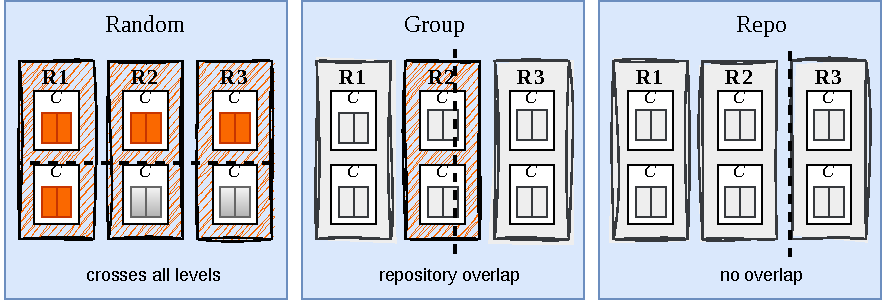
\includegraphics[width=\textwidth]{split.pdf}
\caption{What each protocol permits to cross the train/test boundary. Three
repositories (R1--R3), each holding commits (C), each holding a vulnerable
function and its patched counterpart. Hatching marks material appearing on both
sides of the split. All three protocols partition the identical corpus; only
the level at which the cut is made changes.}
\label{fig:split}
\end{figure}

\subsubsection{Audited disjointness}
Every split ships an audit over four keys. Table~\ref{tab:audit} reports them;
the \texttt{random} row is what a plain stratified shuffle admits.

\begin{table}[h]
\centering
\caption{Train/test overlap by key. The \texttt{random} row is the control.}
\label{tab:audit}
\begin{tabular}{lrrrr}
\toprule
\textbf{Protocol} & \textbf{repo} & \textbf{commit} & \textbf{pair} & \textbf{clone} \\
\midrule
\texttt{repo}   & 0 & 0 & 0 & 0 \\
\texttt{group}  & 197\rlap{$^\dagger$} & 0 & 0 & 0 \\
\texttt{random} & 626 & 3,717 & 1,590 & 3,186\rlap{$^\ddagger$} \\
\bottomrule
\end{tabular}
\begin{tablenotes}\footnotesize
\item $^\dagger$ By design: \texttt{group} does not separate repositories.
\item $^\ddagger$ \texttt{random} is built without clone-family atomicity, since
it is the control, so its clone overlap is measured after the fact rather than
enforced. 3,771 test functions belong to a family that also appears in training.
\item Under \texttt{random}, 1,590 functions appear in training alongside their
own patched counterpart in test: the same function, differing by the fix, with
the opposite label.
\end{tablenotes}
\end{table}


\subsection{Models and controls}
All model backbones use identical node features (GraphCodeBERT embeddings of each node's code, concatenated with a learned node-type embedding), as well as identical pooling, loss function, optimizer, folds, and metrics. Only the specified component varies. Each node is described by two concatenated vectors: a 768-dimensional GraphCodeBERT~\citep{guo2021graphcodebertpretrainingcoderepresentations} embedding of its code, truncated at 128 tokens, and a 64-dimensional learned embedding of its syntactic type. Each edge carries a 32-dimensional learned embedding of its relation type.

\begin{description}[leftmargin=1.2em,itemsep=2pt]
  \item[Architectures] Graph Attention Network (GAT)~\citep{DBLP:conf/iclr/VelickovicCCRLB18}, Graph Convolutional Network (GCN)~\citep{Kipf2016SemiSupervisedCW}, Graph Isomorphism Network (GIN)~\citep{xu2018how} and a Graph Transformer~\citep{3454287.3455360,shi2021masked}, spanning attention, spectral convolution, sum aggregation and global attention. All are the reference implementations in PyTorch Geometric~\citep{fey2019fast}; the typed-edge condition uses its relational convolution~\citep{schlichtkrull2018modeling} where the operator has no edge-feature term.
  \item[\texttt{no graph}] Every edge deleted; depth, width and pooling unchanged. Isolates structure from text.
  \item[\texttt{untyped}] All four CPG relation types (AST, CFG, DDG, CDG) collapsed to one. Isolates edge-type information.
  \item[\texttt{type-only}] Node text zeroed; the model sees the graph and each node's syntactic kind but never an identifier or literal.
  \item[\texttt{topology}] Text zeroed and node types collapsed. Nothing survives but graph shape. This is the floor, and it is what makes a non-zero \texttt{type-only} result interpretable, since graph size alone correlates with the label.
  \item[bag-of-words] Node features replaced with hashed token counts at identical width. A weak-encoder control for the objection that strong features leave the graph nothing to add.
\end{description}


\subsection{Metrics}
ROC-AUC is reported as the primary metric because it is invariant to prevalence, which varies across protocols. Since macro-F1 alone is insufficient for evaluating a detector at a realistic base rate, PR-AUC, MCC, false-positive rate, and recall at fixed false-positive budgets are also reported, each referenced against its partition's prevalence.

\subsection{Reporting variance}
\label{sec:variance}
Run-to-run standard deviation on this task is approximately $0.010$, which is comparable to the magnitude of several measured effects. Principal results are reported over five seeds when the claim depends on a small difference, and over three seeds otherwise, with the count specified, and differences are tested rather than read off the means~\citep{arcuri2011practical}. Each run also records per-fold test scores. Section~\ref{sec:variance-result} demonstrates the importance of this approach: every single-seed estimate reported there disagrees with its five-seed mean, one of them by a factor of twenty-eight, and individual seeds disagree with the mean in sign in all three cases.

\section{Results}
\label{sec:results}

\subsection{The split protocol accounts for most reported performance (\textbf{RQ1})}
\label{sec:ladder}

Table~\ref{tab:ladder} isolates the effect of test partition overlap with training by holding corpus, architecture, node features, folds, and seeds constant.

\begin{table}[h]
\centering
\caption{GAT backbone. All variables except the data
split are held constant: corpus, architecture, node features, folds and seeds
remain unchanged. The \texttt{random} protocol is the standard in existing
literature.}
\label{tab:ladder}
\begin{tabular}{lccc}
\toprule
& \multicolumn{2}{c}{\textbf{ROC-AUC}} & \\
\cmidrule(lr){2-3}
\textbf{Protocol} & \textbf{five-fold} & \textbf{single model} & \textbf{seeds} \\
\midrule
\texttt{random} & $0.796 \pm 0.002$ & $0.774 \pm 0.004$ & 5 \\
\texttt{group}  & $0.657 \pm 0.008$ & $0.702 \pm 0.008$ & 4\rlap{$^\dagger$}/5 \\
\texttt{repo}   & $0.585 \pm 0.012$ & $0.649 \pm 0.012$ & 5 \\
\midrule
leakage share   & $71.5\%$          & $45.5\%$          & \\
\bottomrule
\end{tabular}
\begin{tablenotes}\footnotesize
\item $^\dagger$ One \texttt{group} seed is excluded. It could not be trained at
the batch size used everywhere else, and the reduced-batch rerun is not
comparable: repeating a different seed at that batch size costs $0.059$ ROC-AUC.
\end{tablenotes}
\end{table}

\begin{figure}[h]
\centering
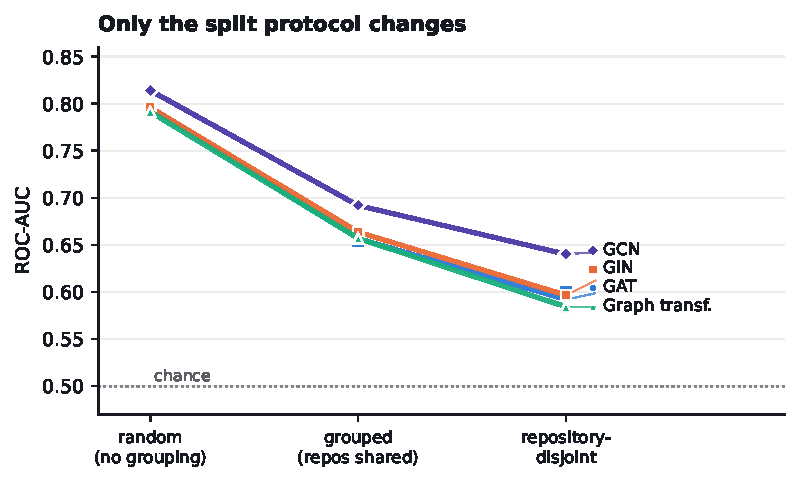
\includegraphics[width=\columnwidth]{ladder.pdf}
\caption{Four graph backbones under the three split protocols. Corpus, node
features, folds and seeds are held fixed; the only thing that varies is what
the test partition is permitted to share with training. All four decline by a
similar amount, and their ordering is broadly preserved, so the effect is a
property of the protocol rather than of any one architecture.}
\label{fig:ladder}
\end{figure}

Figure~\ref{fig:ladder} illustrates the decline across all backbones. Shares
are taken against the margin above chance, not against the raw score: under the
five-fold procedure that margin is $0.796-0.5=0.296$, and the drop to the
repository-disjoint score is $0.796-0.585=0.211$, so
$0.211/0.296 = \textbf{71.5\%}$ of the usable signal is attributable to what the
split permits. Of that margin, \textbf{47.0\%} is due to duplicates, patched
twins and shared commits, \textbf{24.4\%} to repository overlap, and
\textbf{28.5\%} survives every control. The last figure is what remains, not a
further component of the loss.

The second column of Table~\ref{tab:ladder} is the reason this paper reports
two procedures throughout. Holding the corpus, architecture, features and seeds
fixed and changing only whether the reported model is a five-fold ensemble or a
single model trained on the whole partition moves the repository-disjoint score
from $0.585$ to $0.649$ and the leakage share from $71.5\%$ to $45.5\%$. Both
are defensible procedures and neither is stated in the papers we surveyed.
Section~\ref{sec:procedure} examines why they differ.

The $0.796$ ROC-AUC aligns with values commonly reported in the literature, and was achieved without any modifications to the model.

\subsubsection{Replication across architectures}
Table~\ref{tab:arch} extends the analysis to four architectures representing different aggregation mechanisms: attention, spectral convolution, sum aggregation, and global attention as implemented in a graph transformer.

\begin{table}[h]
\centering
\caption{Four architecture families under the repository-disjoint protocol,
five seeds per cell, reported under both training procedures. The ordering of
the architectures differs between the two columns and the spread collapses from
$0.044$ to $0.009$, so architecture comparisons in this setting are not
separable from the training procedure.}
\label{tab:arch}
\begin{tabular}{lccc}
\toprule
\textbf{Backbone} & \textbf{five-fold} & \textbf{single model} & \textbf{difference} \\
\midrule
GAT               & $0.585 \pm 0.012$ & $0.649 \pm 0.012$ & $+0.065$ \\
GCN               & $0.628 \pm 0.008$ & $0.653 \pm 0.008$ & $+0.025$ \\
GIN               & $0.591 \pm 0.009$ & $0.658 \pm 0.015$ & $+0.067$ \\
Graph transformer & $0.587 \pm 0.007$ & $0.650 \pm 0.010$ & $+0.064$ \\
\bottomrule
\end{tabular}
\end{table}

Every architecture gains from the single-model procedure, three of them by
about $0.065$, and all four differences are significant. GCN is the exception at
$+0.025$; we have no account of why and report it as an observation.

Two things in this table bear on how architecture comparisons in this area
should be read. The ordering changes: GCN is strongest under the ensemble and
GIN under the single model. And the spread across four families collapses from
$0.044$ to $0.009$, which is within the seed standard deviation of the
individual cells. Under the better procedure these architectures are not
distinguishable from one another, so a comparison between them is reporting the
training procedure at least as much as the aggregation scheme. GIN is a useful
case: it is the most expressive of the four under the 1-Weisfeiler-Lehman
criterion, unlike GCN and GAT, and it is third of four under one procedure and
nominally first under the other, by a margin smaller than noise. This motivates
the analysis in Section~\ref{sec:graph-worth}.

\subsection{The encoding sets what the graph is measured to be worth (\textbf{RQ2})}
\label{sec:graph-worth}

The protocol above fixes what is being measured. Within it we vary how the
graph is presented to the network, holding the corpus, the architecture, the
node features and the training schedule constant. Two encoding choices are
available and neither is varied in this literature. One of them changes the
measured contribution of the graph by more than most published architectural
improvements; the other changes nothing at all. Which is which is not
predictable from how meaningful the choice sounds.

\subsubsection{Edge relation types}
Joern labels each edge with the relation it represents: abstract syntax, control
flow, data dependence or control dependence. Collapsing those four labels into a
single undifferentiated relation, while leaving the connectivity untouched,
isolates what the labels are worth.

The comparison must hold edge direction fixed. Because reversed edges are
encoded as additional relation types (Section~\ref{sec:method}), collapsing the
labels in a directed graph and in a bidirectional one are different
interventions, and an unmatched pair confounds the two. Both arms below are
bidirectional; connectivity is identical, and only the distinguishability of the
four relations varies.

\begin{table}[h]
\centering
\caption{Effect of relation labels, five seeds per cell, repository-disjoint.
Both arms bidirectional, so direction is held fixed and only the four relation
labels vary. Seed standard deviations are $0.005$--$0.012$ throughout; the GIN
row is discussed below.}
\label{tab:typed}
\small
\begin{tabular}{lcccc}
\toprule
\textbf{Backbone} & \textbf{typed} & \textbf{collapsed} & \textbf{effect} & \textbf{95\% CI} \\
\midrule
GAT         & $0.618$ & $0.620$ & $-0.002$ & $[-0.012,+0.007]$ \\
GCN         & $0.634$ & $0.624$ & $+0.010$ & $[-0.007,+0.026]$ \\
G.\ transf. & $0.603$ & $0.603$ & $-0.001$ & $[-0.022,+0.021]$ \\
\midrule
GIN$^\dagger$ & $0.583$ & $0.589$ & $-0.006$ & $[-0.015,+0.004]$ \\
\bottomrule
\end{tabular}
\begin{tablenotes}\footnotesize
\item $^\dagger$ Cannot read relation labels; true effect is zero by
construction.
\end{tablenotes}
\end{table}

\noindent Pooled over the three architectures whose operators condition on
relation type, distinguishing data dependence from syntactic containment is
worth $+0.002$ ROC-AUC (95\% CI $-0.005$ to $+0.010$, $n=15$). An equivalence
test against a margin of $0.033$, the size of the edge-direction effect below,
rejects an effect of that magnitude at $p<10^{-6}$. The labels are not merely
unproven here; they are bounded to within a third of the run-to-run standard
deviation.

The GIN row establishes what that bound means. Its operator sums over
neighbours with no edge-feature term, so the typed and collapsed conditions are
the same model and the true difference is exactly zero. It nonetheless measures
$-0.006$, with individual seeds ranging from $+0.006$ to $-0.012$, which is the
floor imposed by nondeterministic accumulation in scatter operations. No
architecture departs from that floor.

This is the one place where an unmatched comparison would have produced a
different answer. Against a \emph{directed} collapsed baseline the same typed
model appears to gain $+0.024$, but that figure is the edge-direction effect of
Section~\ref{sec:direction} arriving through the relation table, not a property
of the labels.

\begin{figure}[htb]
\centering
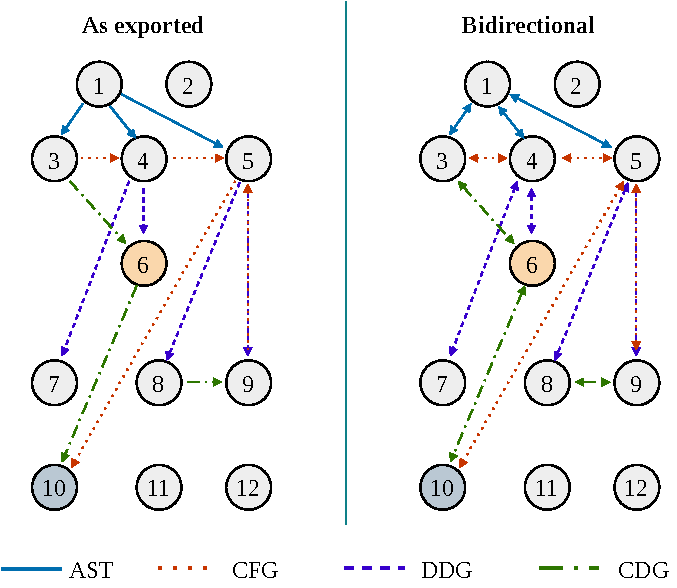
\includegraphics[width=0.85\textwidth]{direct.pdf}
\caption{The same code property graph under both encodings. Edge styles
distinguish the four relations. On the left the edges run in the direction the
exporter emits them, so a node aggregates only from its predecessors. On the
right each edge is additionally traversable in reverse, entered as a distinct
relation type rather than by making the graph undirected, so an operator that
reads the relation label can still tell a forward traversal from a backward
one.}
\label{fig:direction}
\end{figure}

\subsubsection{Edge direction}
\label{sec:direction}
Joern exports the code property graph as a directed object, and the pipeline
above consumes it unaltered. Figure~\ref{fig:direction} contrasts the two
encodings on one graph. A node therefore aggregates only from its
predecessors: an abstract-syntax parent never receives from its children, and a
definition never receives from its uses. Measured over 767 graphs, the average
node reaches only $18.9\%$ of its own function within three layers under this
convention, against $73.8\%$ once each edge is also traversable in the opposite
direction. Widening the receptive field by adding layers instead would incur the
costs this narrows away from~\citep{li2018deeper,alon2021bottleneck}.

Adding every edge back as a distinct reversed relation, which leaves the
parameter count unchanged because the relation table already had unused
capacity, changes the picture materially:

\begin{center}
\small
\begin{tabular}{lccc}
\toprule
\textbf{Protocol} & \textbf{directed} & \textbf{bidirectional} & \textbf{gain ($p$)} \\
\midrule
\texttt{random} & $0.796$ & $0.793$ & $-0.003$ (0.014) \\
\texttt{group}  & $0.657$ & $0.666$ & $+0.009$ (0.286) \\
\texttt{repo}   & $0.585$ & $0.618$ & $+0.033$ (0.012) \\
\bottomrule
\end{tabular}
\end{center}

\noindent All $p$-values are paired $t$-tests over five seeds, the seed being
the unit of replication. The five folds inside a run share a training partition
and a seed and are not independent, so pooling them would inflate the sample
fivefold.

The gain appears only as the protocol tightens. Under \texttt{random}
the reverse direction is slightly harmful, under \texttt{group} it does not
reach significance, and under repository-disjoint evaluation it is worth
$+0.033$ ($p=0.012$). That ordering is consistent with the rest of this section: when
duplicates and patched twins are available, token content alone suffices and
improved structural reach adds nothing. The change is measurable precisely where
generalisation is.

The benefit tracks whether the operator can read the relation label, and it
does so exactly. Repeated at five seeds under the repository-disjoint protocol:

\begin{center}
\small
\begin{tabular}{lcccc}
\toprule
& \textbf{directed} & \textbf{bidirectional} & \textbf{gain} & \textbf{$p$} \\
\midrule
GAT         & $0.585$ & $0.618$ & $+0.033$ & 0.012 \\
G.\ transf. & $0.587$ & $0.603$ & $+0.016$ & 0.010 \\
GCN         & $0.628$ & $0.634$ & $+0.006$ & 0.062 \\
\midrule
GIN         & $0.591$ & $0.583$ & $-0.008$ & 0.043 \\
\bottomrule
\end{tabular}
\end{center}

\noindent Two of the three operators that condition on edge type gain
significantly, GAT by $0.033$ and the graph transformer by $0.016$. GCN gains
$0.006$ at $p=0.062$, which does not establish an effect and we do not count it
as one. GIN, the only operator that cannot read the relation label, is the sole
architecture significantly harmed. The mechanism is direct.
Reversed edges enter as distinct relation types, so an operator that reads the
relation gains the ability to tell a forward traversal from a backward one,
while GIN sums over neighbours with no edge-feature term and receives only a
doubled adjacency it cannot distinguish from the forward graph. We verified
this by relabelling the edge types of a fixed graph, which leaves GIN's output
bit-identical while changing the output of the other three.

This result does not survive a change of training procedure, and that is the
most important thing about it. Repeating the same comparison with a single
model trained on the whole partition, five seeds on each side:

\begin{center}
\small
\small
\begin{tabular}{lcccc}
\toprule
\textbf{Procedure} & \textbf{directed} & \textbf{bidir.} & \textbf{gain} & \textbf{$p$} \\
\midrule
five-fold ensemble & $0.585$ & $0.618$ & $+0.033$ & 0.012 \\
single model       & $0.649$ & $0.643$ & $-0.006$ & 0.41 \\
\bottomrule
\end{tabular}
\end{center}

\noindent The direction of the edges is worth a third of a standard deviation
of nothing once the model is trained the better way, and the better way is also
the stronger one: the worst single-model configuration here exceeds the best
five-fold configuration. The reading we take is not that edge direction is
useless, nor that it is valuable, but that its measured value is contingent on
a choice that no paper in this area reports. An ablation of this kind cannot be
interpreted without the training procedure stated alongside it.

A plausible mechanism ties the two together. The five-fold ensemble's reach
over the graph is limited by what each member learns from four fifths of the
data with an epoch chosen on repositories it has already seen; widening the
receptive field compensates for part of that. A single model trained on the
whole partition does not need the compensation. We do not test this directly
and offer it as an interpretation rather than a result.

\subsubsection{Removing node text}
With text zeroed, leaving node types and graph structure, ROC-AUC is:

\begin{center}
\begin{tabular}{lcc}
\toprule
& \multicolumn{2}{c}{\textbf{ROC-AUC}} \\
\cmidrule(lr){2-3}
& \texttt{random} & \texttt{repo} \\
\midrule
\texttt{type-only} (no text) & 0.714 & 0.476 \\
\texttt{topology} (shape only) & 0.452 & 0.494 \\
\bottomrule
\end{tabular}
\end{center}

Node types alone do not indicate vulnerabilities; for example, the presence of three \texttt{CALL} nodes and two \texttt{IDENTIFIER}s does not reveal a buffer overflow. However, they serve as structural fingerprints. The $0.714$ ROC-AUC under a random split reflects recognition of previously encountered structures rather than true vulnerability detection, and this value surpasses those reported by several published systems. In contrast, under a repository-disjoint split, the same model performs at chance. The \texttt{topology} result establishes the baseline and eliminates function length as a confounding factor, as the MCC is exactly $0.000$.

\begin{figure}[htb]
\centering
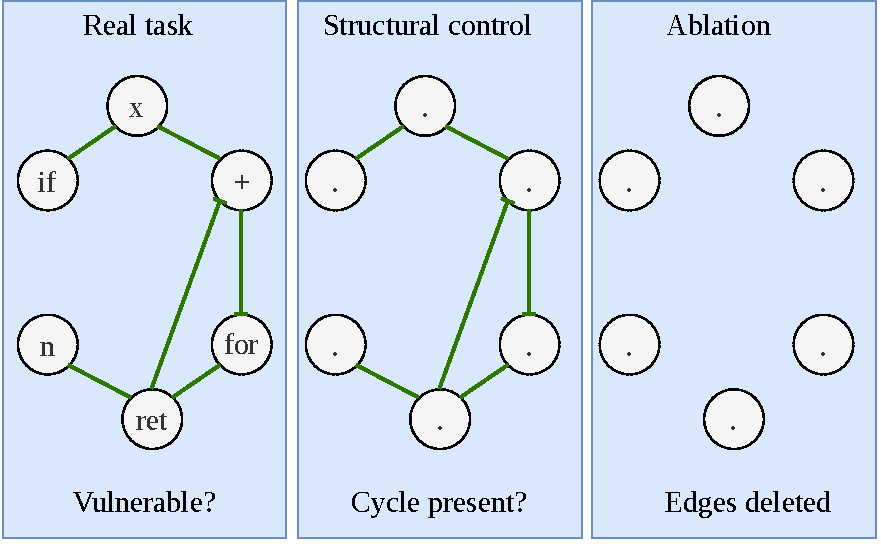
\includegraphics[width=\textwidth]{control.pdf}
\caption{The positive control. Left: the real task, with node text and the
vulnerability label. Centre: the same graphs with node content replaced by
noise and node types collapsed, labelled by a property computable from the edge
set alone. Right: the same again with the edges deleted, which leaves only
graph size. The evidence is the gap between the centre and right conditions.}
\label{fig:control}
\end{figure}

\subsubsection{A positive control for structural learning}
The \texttt{topology} row above is open to two readings. It may mean that graph
shape carries no vulnerability signal, or it may mean that this pipeline cannot
read graph shape at all. Those are competing explanations for the same number,
and the ablations reported so far do not separate them.

The following control does, and Figure~\ref{fig:control} sets out its three
conditions. The graphs are the same real code property graphs, but every node
feature is replaced with random noise and every node type is collapsed to a
single identifier, so nothing about a node carries information.
The labels are chosen to be computable from the edge set alone, which places
them within what message passing of this family can in principle
express~\citep{xu2018how,morris2019weisfeiler}.
The label is then computed from the edge set alone: whether the control-flow
subgraph contains a directed cycle, and whether data-dependence edges outnumber
control-flow edges. A model that can read structure must exceed chance; a model
with the edges deleted retains only the node count.

\begin{center}
\small
\begin{tabular}{lccc}
\toprule
\textbf{Structural label} & \textbf{graph} & \textbf{no graph} & \textbf{gain} \\
\midrule
CFG contains a cycle     & $0.860$ & $0.756$ & $+0.104$ \\
DDG edges $>$ CFG edges  & $0.976$ & $0.673$ & $+0.303$ \\
\bottomrule
\end{tabular}
\end{center}

\noindent Three seeds each. The evidence here is the \emph{gain}, not the
absolute score, and the distinction matters because the edge-free column is far
above chance: $0.756$ for loop presence and $0.673$ for the edge-type ratio.
Both labels are therefore substantially predictable from graph size alone, which
pooling exposes and which both columns share equally. Nothing about the $0.860$
should be read as evidence that the model has understood control flow.

What the comparison does establish is that deleting the edges costs the model
something on a label defined by the edges, $+0.104$ and $+0.303$ on the same
graphs with the same architecture. The second of these is the stronger
instrument: an edge-type ratio is less predictable from node count than loop
presence is, and the gain is three times larger. A pipeline that could not read
the edge set at all would show no gain on either.

Two limits are worth stating. Loop presence and edge-type ratios are coarse,
global properties, and success on them does not establish that the model could
localise a subtle dependency change. And the control shows that the apparatus
can extract edge information, not that the vulnerability label depends on edge
information; those are different claims and only the first is tested here.

\subsection{What the graph representation captures (\textbf{RQ3})}
\label{sec:mechanism}

The encoding choices above recover a contribution of the same order as the
pretrained encoder, and the natural next question is what that recovered signal
consists of. This section asks what the network is doing with the graph it is
given, by
instrumenting a trained model rather than by running further ablations. The
question is not whether the graph helps, which
Section~\ref{sec:graph-worth} measures, but which capabilities the resulting
representation does and does not support.

Deleting the edge set from a trained model at inference, leaving its weights
untouched, isolates the contribution message passing makes to the representation
the classifier consumes. This is instrumentation, not an ablation: no model is
retrained, and the comparison is between two forward passes of the same
network.

Fix a trained GAT and write
\[
  z_G = \operatorname{pool}\bigl(\mathrm{GNN}(X, E)\bigr), \qquad
  z_0 = \operatorname{pool}\bigl(\mathrm{GNN}(X, \varnothing)\bigr)
\]
for the pooled representation the classifier consumes, computed with the real edge set and with the edges deleted under \emph{identical weights}. We report both split protocols; each uses its own independently trained model.

\subsubsection{The network is not over-smoothed}
The standard mechanical explanation for a graph network behaving like a graph-free one is over-smoothing: repeated aggregation acts as a low-pass filter, node representations converge toward a common direction, and any permutation-invariant readout then returns approximately that direction. The diagnostic is the Dirichlet energy over $ L_2$-normalized rows,
\[
E(H) ;=; \frac{1}{|E|}\sum_{(i,j) \in E}
\Bigl| \tfrac{h_i}{|h_i|} - \tfrac{h_j}{|h_j|} \Bigr|^2 ,
\]
which vanishes exactly when message passing has collapsed the representation.

\begin{center}
\begin{tabular}{lcccc}
\toprule
& \multicolumn{2}{c}{\texttt{repo}} & \multicolumn{2}{c}{\texttt{random}} \\
\cmidrule(lr){2-3}\cmidrule(lr){4-5}
& $E(H)$ & pairwise $\cos$ & $E(H)$ & pairwise $\cos$ \\
\midrule
input & $1.342$ & $0.236$ & $1.350$ & $0.231$ \\
GAT 1 & $1.002$ & $0.208$ & $1.038$ & $0.202$ \\
GAT 2 & $0.794$ & $0.246$ & $0.857$ & $0.215$ \\
GAT 3 & $0.643$ & $0.281$ & $0.667$ & $0.266$ \\
\bottomrule
\end{tabular}
\end{center}

Energy decreases by factors of $2.09$ and $2.03$ across the two protocols, but does not approach zero. The mean pairwise cosine similarity between node representations remains between $0.20$ and $0.29$ throughout, decreasing at the first layer and then increasing, ending only $0.045$ and $0.035$ above the initial value for each protocol. These values are far from the near-unity similarity that would indicate collapse. With three layers and median test graph sizes of $75$ and $49$ nodes, the network is not in a collapsed regime. \textbf{Over-smoothing does not account for the observed results}, and neither reducing network depth nor adopting a differentiated propagation scheme would recover the missing performance. All reported quantities are measured on a single trained network per protocol over the entire test partition.

\subsubsection{The edges are used, not ignored}
The network also does not ignore the graph structure. Removing edges from the trained model results in a substantial change in the pooled representation: the mean $\cos(z_G, z_0)$ is $0.726$ for \texttt{repo} and $0.574$ for \texttt{random}, with only $1.4\%$ and $2.4\%$ of graphs, respectively, exceeding $0.99$. This indicates that message passing significantly alters the representation.

How much of that work is new? Fitting a ridge map $W$ on the training partition and decomposing the test representation as $z_G = W z_0 + r$ separates the part recoverable from the edge-free features from the part that is not. The map attains $R^2 = 0.719$ and $0.683$, so roughly $70\%$ of the graph representation
is a linear re-encoding of information already present in the pooled node features. The residual component is substantial: $|r| / |z_G|$ equals $0.4475$ and $0.4506$. The close agreement between the two protocols and the two independently trained models (within $0.004$) suggests that this value reflects the inherent geometry of message passing on these graphs, rather than being an artifact of a particular run.

\subsubsection{What the transformation is worth}
Whether that new component carries anything the classifier can use is a conditional question, and $r$ cannot answer it directly: subtracting a ridge fit removes linear predictability from $z_0$ rather than information, so a probe on $r$ alone conflates novelty with re-encoding. Holding the probe class fixed, we compare instead what each representation supports: $\Delta = \text{ROC-AUC}(z_G) - \text{ROC-AUC}(z_0)$.

\begin{center}
\begin{tabular}{lccc}
\toprule
& $z_0$ & $z_G$ & $\Delta$ \\
\midrule
\multicolumn{4}{l}{\emph{\texttt{repo}}} \\
linear             & $0.5814$ & $0.5991$ & $+0.018$ \\
MLP                & $0.5792$ & $0.5780$ & $-0.001$ \\
gradient boosting  & $0.5750$ & $0.6020$ & $+0.027$ \\
\midrule
\multicolumn{4}{l}{\emph{\texttt{random}}} \\
linear             & $0.7698$ & $0.7793$ & $+0.010$ \\
MLP                & $0.7783$ & $0.7783$ & $-0.000$ \\
gradient boosting  & $0.7804$ & $0.7953$ & $+0.015$ \\
\bottomrule
\end{tabular}
\end{center}

The MLP results should not be interpreted as null findings: the seed standard deviation for $z_G$ is $0.006$ and $0.011$, placing $\Delta$ within the range of measurement noise. Additionally, on \texttt{repo}, the MLP does not match the performance of a linear probe on the same input. Gradient boosting provides more stable results, with seed standard deviations between $0.0007$ and $0.0028$, and yields positive values under both protocols. Selecting the best probe for each representation results in $+0.021$ on \texttt{repo} and $+0.015$ on \texttt{random}.

The graph therefore contributes information that is not recoverable from the node features alone. This estimate is independent of the end-to-end ablation of Section~\ref{sec:graph-worth}, which retrains from scratch rather than probing a fixed representation. On \texttt{repo}, the two are close, $+0.014$ retrained against $+0.021$ probed; on \texttt{random}, they are not, $+0.003$ against $+0.015$.

The probe results should be interpreted as upper bounds. In this context, $z_0$ is not derived from a properly trained graph-free model; rather, it is obtained by removing edges at inference from a network trained with edge information, resulting in weights adapted to inputs that are no longer present. This mismatch artificially inflates $\Delta$ relative to a fair comparison in which a graph-free model is trained independently. The retrained ablation provides a more accurate measurement, while the probe quantifies the maximum potential contribution of the graph.

\subsubsection{Discrimination within vulnerable/patched pairs}
A natural objection to the aggregate figures is that they average over easy
cases. Swapping two statements can alter control or data flow while leaving the
node set almost unchanged, and such a case must depend on structure; a test
partition dominated by unrelated safe functions would hide it. We therefore
evaluate on the $2{,}067$ vulnerable/patched pairs held entirely within the test
partition, scoring a model correct when it ranks the vulnerable member above its
own patched twin. Project identity, length and style cancel within a pair. Pairs
are split by whether node text is near-identical (Jaccard $\geq 0.95$), which
isolates the cases where structure is the only difference.

\begin{center}
\begin{tabular}{lccc}
\toprule
\textbf{Slice} & \textbf{pairs} & \textbf{graph} & \textbf{no graph} \\
\midrule
structure only & $165$  & $0.502$ & $0.388$ \\
text differs   & $1{,}341$ & $0.469$ & $0.467$ \\
\bottomrule
\end{tabular}
\end{center}

\noindent Five seeds. The graph is worth $+0.114$ ($p=0.038$) on the
structure-only slice and nothing at all where text also differs ($+0.001$,
$p=0.98$), and the contrast between the two slices is itself significant
($p=0.024$). The aggregate metric does dilute a real, slice-specific effect.

The absolute values matter more than the difference. On the structure-only
slice the graph model reaches $0.502$, which is chance, while the edge-free
model is anti-correlated at $0.388$. Adding edges removes a systematic error
rather than conferring skill. Repeating the measurement with the bidirectional
encoding of Section~\ref{sec:graph-worth} leaves this unchanged: $0.497 \pm
0.033$ against $0.502 \pm 0.057$ over the same five seeds ($p=0.85$), and the
bidirectional model is itself indistinguishable from chance ($p=0.85$ against
$0.5$). The encoding that recovers the largest aggregate gain in this paper
recovers nothing here. \textbf{No configuration we tested distinguishes a
vulnerable function from its own patch at better than chance}, which is
consistent with the paired evaluation of PrimeVul~\citep{ding2024primevul} and
is the sharper form of this paper's claim.

\subsubsection{Reading}
Three properties of the trained model fit together. It is not over-smoothed, it
does use its edges, and message passing induces a large geometric change in the
pooled representation. Yet on the discrimination that matters, separating a
function from its own patch, no configuration exceeds chance.

The encoding results of Section~\ref{sec:graph-worth} are therefore real, and
bounded in a specific way. Restoring edge direction and preserving relation
labels each recover aggregate ROC-AUC, and the instrumentation here indicates
what that recovered signal does and does not support: the representation the network builds from the graph
separates vulnerable from safe functions in aggregate, without localising the
defect that distinguishes a function from its fix.

We are explicit about what this does not establish. It does not show that code
property graphs cannot support that capability, only that this pipeline's
representation does not. One plausible account is that a function-level graph
omits the interprocedural flow many real vulnerabilities depend on, so the
structure available at this scope is thin; testing that requires a different
experiment than the ones reported here, and we do not claim it.

\subsection{Calibrating the protocol against a published model (\textbf{RQ4})}
\label{sec:linevul}

Every measurement so far is internal to one pipeline, which leaves one
alternative explanation open: that the repository-disjoint partition is simply
too hard, or the corpus too noisy, for any model to do well on. If that were so,
the encoding effects reported above would be differences between degrees of
failure rather than measurements of anything. An external model settles it.
LineVul~\citep{fu2022linevul} is a published token-based detector that fine-tunes
CodeBERT on raw function text and uses no graph. We ran the authors'
implementation unmodified, adding only a prediction-score dump, on the identical
splits. Table~\ref{tab:linevul} reports the result.

\begin{table}[h]
\centering
\caption{Official LineVul (authors' code) on the same splits and the same test
partitions as our graph models. Seed coverage as in Table~\ref{tab:arch}: the
\texttt{repo} column and the leakage share are five-seed means, the other
columns single runs except for GAT. The purpose is to establish that the
repository-disjoint partition carries learnable signal, and to compare how much
of each model's performance depends on the protocol.}
\label{tab:linevul}
\begin{tabular}{lcccc}
\toprule
& \multicolumn{3}{c}{\textbf{ROC-AUC}} & \textbf{leakage} \\
\cmidrule(lr){2-4}
& \texttt{random} & \texttt{group} & \texttt{repo} & \\
\midrule
GAT (graph)          & 0.796 & 0.657 & 0.585 & 71.4\% \\
GCN (graph)          & 0.814 & 0.692 & 0.628 & 59.2\% \\
GIN (graph)          & 0.796 & 0.664 & 0.591 & 69.3\% \\
\textbf{LineVul (no graph)} & \textbf{0.914} & \textbf{0.856} & \textbf{0.792} & \textbf{29.5\%} \\
\bottomrule
\end{tabular}
\end{table}

\noindent The first thing this establishes is that the partition is not
degenerate. A published model reaches $0.792$ ROC-AUC on the same
repository-disjoint test functions, so the corpus and the split carry signal
that a learner can find, and the lower figures reported above are properties of
what was measured rather than of an unlearnable task.

The second is a difference in how much each model depends on the protocol.
Only $29.5\%$ of LineVul's signal above chance is attributable to leakage,
against $59.2$--$71.4\%$ for the graph models; its decomposition is $14.1\%$
duplicates and twins, $15.4\%$ repository overlap, and $70.5\%$ surviving every
control. The ranking of the two approaches under a permissive protocol is
therefore a poor guide to their ranking under a strict one.

We report this as calibration and not as a verdict, for two reasons. LineVul
fine-tunes its encoder end to end while the graph models here consume frozen
features, so any absolute difference mixes representation with training regime
(Section~\ref{sec:threats}). And the published graph detectors were not run, so
nothing here bounds what a different graph pipeline could achieve; what
Section~\ref{sec:graph-worth} shows is that at least one encoding choice in our
own was leaving signal unused.

\subsubsection{Training procedure}
\label{sec:procedure}
Everything above is reported under one training configuration: a five-fold
ensemble, each member trained on four fifths of the training partition with the
library defaults inherited from the stage-1 pipeline. That configuration is a
choice, and this section measures what the choice is worth. It is the largest
effect in this paper.

Two factors are confounded in any naive comparison and we separate them. The
first is \emph{ensembling}: five models on four fifths each, averaged, against
one model on the whole partition. The second is the \emph{recipe}: the epoch
budget, effective batch size, learning rate and schedule. Holding the recipe
fixed and varying only the first gives a $2\times2$ with five seeds per cell:

\begin{table}[h]
\centering
\caption{Ensembling and recipe, separated. All cells are GAT, bidirectional,
repository-disjoint, five seeds, selecting the epoch on the same held-out
validation partition. The default recipe is the stage-1 inheritance (120
epochs, batch 256, plateau decay); the selected recipe is described below.}
\label{tab:procedure}
\small
\begin{tabular}{lcc}
\toprule
& \textbf{default recipe} & \textbf{selected recipe} \\
\midrule
one model, whole partition & $0.585 \pm 0.018$ & $0.650 \pm 0.004$ \\
five-fold ensemble         & $0.618 \pm 0.010$ & $0.649 \pm 0.004$ \\
\bottomrule
\end{tabular}
\end{table}

\noindent Three things follow. Ensembling is worth $+0.033$ ($p=0.007$) under
the default recipe and $-0.002$ ($p=0.59$) under the selected one, so it is not
a property of the method but a compensation for undertrained members. The extra
fifth of training data is worth $+0.003$ ($p=0.73$) and can be set aside. And
the recipe is worth $+0.032$ ($p=0.0001$) measured between the best cell
available under each, which is larger than any representational effect reported
in this paper.

\paragraph{How the recipe was selected.} A comparison of two recipes is only
evidence if neither was chosen on the test set. We therefore fixed the
alternative by grid search on the validation partition alone: epoch budget
$\{15, 30\}$, effective batch $\{128, 256\}$, learning rate
$\{10^{-3}, 5\times10^{-4}, 2\times10^{-4}\}$, twelve configurations, ranked by
validation ROC-AUC with the test partition untouched until the ranking was
fixed. The selected configuration is 30 epochs, effective batch 128, learning
rate $2\times10^{-4}$, re-run at five seeds for the figure above.

That search carries its own finding. Across the twelve configurations,
validation ROC-AUC spans $0.015$ while test spans $0.029$, and the rank
correlation between them is weak ($\rho=0.32$, $p=0.31$). Selecting on
validation returns a test score of $0.650$; the best test score in the grid is
$0.661$, at a configuration ranked seventh on validation. Honest selection
therefore leaves roughly a point of ROC-AUC unreachable, and a reported figure
near the top of that range is more likely to reflect selection on test than a
better method. We note the limitation that the grid uses one seed per cell, and
the seed standard deviation at this protocol is about a third of the test range
it spans, so the spread should be read as an upper bound on recipe sensitivity
rather than a point estimate.

\subsection{Absolute performance}
At a 1\% false-positive rate, the graph pipeline's recall under the
repository-disjoint protocol is \textbf{$0.016$}: it finds about two of every
hundred vulnerable functions at an alert volume a reviewer would tolerate. On
the identical test partition, LineVul's recall at the same false-positive rate
is \textbf{$0.278$}, seventeen times higher. Aggregate figures for the graph
pipeline are ROC-AUC $0.585 \pm 0.012$ and MCC $0.061 \pm 0.008$. For ten-way CWE-family classification, macro-F1 is $0.093$, below the $0.100$ chance baseline, indicating performance worse than random guessing. During training, validation macro-F1 reaches $0.65$, but drops to $0.40$ on the test set, suggesting the model memorizes training repositories and fails to generalize.

These figures pertain to the graph-based pipeline, not to vulnerability
detection as a whole. On the same corpus and the same repository-disjoint
partition, LineVul reaches ROC-AUC $0.792$ and MCC $0.438$
(Section~\ref{sec:linevul}), against $0.658$ for the strongest graph
configuration we measured, a single-model GIN. The comparison is not
like-for-like in one respect that should be stated plainly: LineVul fine-tunes
CodeBERT end to end, while every graph model here keeps GraphCodeBERT frozen. A strict protocol does not cost every method equally: the token model
retains most of its performance where this pipeline does not. That ordering is consistent with reports that pretrained token models remain competitive with structure-aware ones once evaluation is tightened~\citep{steenhoek2023empiricalstudydeeplearning,li2025revisitingpretrainedlanguagemodels}.

\subsection{Run-to-run variance}
\label{sec:variance-result}
Run-to-run standard deviation is approximately $0.010$ under the \texttt{repo} protocol ($0.011$ with the graph, $0.010$ without), which is comparable to the effect sizes under investigation~\citep{arcuri2011practical,errica2020fair}. The standard deviation is lower under the \texttt{random} protocol ($0.002$), indicating that variability is greatest under the more rigorous protocol. Single-seed measurements in this study proved unreliable in
both directions:

\begin{center}
\begin{tabular}{lccc}
\toprule
\textbf{Contribution (ROC-AUC)} & $n{=}1$ & $n{=}3$ & $n{=}5$ \\
\midrule
GraphCodeBERT, \texttt{repo} & $-0.022$ & $-0.003$ & $-0.001$ \\
bag-of-words, \texttt{repo}  & $+0.024$ & $+0.023$ & $+0.013$ \\
edge types, \texttt{repo}    & $-0.021$ & $-0.011$ & $-0.009$ \\
\bottomrule
\end{tabular}
\end{center}

The first estimate shrinks by a factor of twenty-eight as seeds accumulate; the other two roughly halve. Individual seeds also disagree with the five-seed mean in sign in every row, and in the first row three of the five do. A single run therefore fixes neither the magnitude nor the direction of these effects. Seed counts are reported throughout, and single-run ablations in this literature should be regarded as provisional.


\section{Discussion}
\label{sec:discussion}

\subsection{What the reported numbers measure}
The three protocols differ in one respect, and that respect accounts for roughly
seventy per cent of the signal above chance. A practitioner reading $0.796$ and
a practitioner reading $0.585$ are reading the same model on the same corpus;
only the question being asked has changed. The first asks whether the detector
recognises functions resembling those it was trained on, which is a
well-specified question and not the one deployment poses. The second asks
whether it generalises to repositories it has never seen, which is.

This is not an argument that published numbers are wrongly computed. It is an
argument of the kind made more broadly about machine-learning-based
science~\citep{kapoor2023leakage}: the number alone does not identify which
question was answered, and the difference is large enough to change
conclusions. A benchmark
result reported without a statement of what the test partition was permitted to
share with training is therefore incomplete in a way that a reader cannot detect
or correct. Neither the mechanism nor the remedy is new to software engineering:
near-duplicate code is pervasive on the platforms these corpora are mined
from~\citep{lopes2017dejavu} and inflates model-of-code results when it crosses
the split~\citep{allamanis2019adverse}, and defect prediction established two
decades ago that cross-project evaluation asks a different and harder question
than within-project evaluation~\citep{zimmermann2009cross}. What our measurements
add is the size of the effect for this task and its decomposition into
duplication and repository overlap.

\subsection{Encoding choices are unreported and consequential}
How much a code property graph is measured to contribute is not a property of
the representation alone. It is a joint property of the representation and an
encoding decision that this literature does not vary and does not report.
Holding everything else fixed, restoring the reverse direction of each edge
moves the same graphs from undetectable to $+0.032$ ROC-AUC under
repository-disjoint evaluation, at no cost in model parameters. A second choice
that looks equally consequential, distinguishing the four relation types,
gains $0.002$ against a matched baseline (95\% CI $-0.005$ to $+0.010$).

The second result is worth stating precisely because the encoding it concerns
looks like the more meaningful one. That an edge carries data dependence rather
than syntactic containment is the kind of information a reader expects a code
property graph to supply, and it makes no measurable difference to any of the
three architectures able to read it.

The direction result is the more striking because the cause is mechanical rather
than statistical. Joern emits a directed graph; a network consuming it unaltered
lets each node aggregate only from its predecessors, which leaves the average
node able to reach under a fifth of its own function within three layers. The
fix is one line, and it is not applied because the encoding is treated as a
property of the input rather than as a design decision.

We note the asymmetry this creates in how the field allocates effort. A new
aggregation scheme is a publishable contribution; the orientation of the edges it
aggregates over is a detail of the data loader. On this corpus the second is
worth more than several of the first, and it is worth more than the relation
labels that motivate the representation in the first place. The same asymmetry has been reported for
graph classification generally, where architectural gains narrow substantially
once the surrounding protocol is held fixed~\citep{errica2020fair}.

\subsection{Aggregate metrics and the capability of interest}
The detectors examined here separate vulnerable from safe functions in aggregate
while failing, at chance, to separate a vulnerable function from its own patched
version. Those are different capabilities, and only the first is measured by the
metric the field reports.

The distinction matters for how results are read. A detector that recognises
which functions resemble known-vulnerable code is useful for triage and
prioritisation. A detector that identifies what specifically is wrong with a
function is what the framing of this literature, and its use of terms like
localisation and explanation, implies. Our measurements indicate that
improvements in the first do not imply progress in the second, and that
aggregate ROC-AUC cannot distinguish them. Reporting a paired evaluation
alongside it costs one additional column and closes that gap.

\subsection{Implications for practice}
Three recommendations follow directly from the measurements. Evaluations should
ship an audit of what the split separates, since the cost of omitting one is
both large and currently invisible. Ablations should report seed counts and a test of significance, because
run-to-run variation here is of the same magnitude as the effects being
measured and the appropriate procedures are
well established~\citep{arcuri2011practical}. And studies reporting a null result for a component should include a
positive control establishing that the model can learn a label defined by that
component, without which a null cannot be distinguished from an instrument that
never read it.

A fourth recommendation concerns the training procedure itself. Whether a study
trains a single model or an ensemble, and how it selects the reported epoch, is
worth more than several of the effects such studies report, and is rarely
stated. We found that selecting the epoch on data sharing repositories with the
training set costs ROC-AUC under a repository-disjoint protocol, which is the
same leakage the split is designed to prevent, reappearing inside the training
loop. That model validation technique is itself a first-order determinant of
reported performance is a finding defect prediction reached
earlier~\citep{tantithamthavorn2017empirical}.

\section{Limitations}
\label{sec:threats}

\subsection{Construct validity}
LineVul fine-tunes its encoder end to end, whereas the principal graph results
use frozen features, so any absolute difference between them mixes
representation with training regime. We attempted to separate the two by training the encoder jointly with the graph network. Against a matched control, identical in data, schedule and architecture but with the encoder frozen, joint training was worth $-0.003$ (paired over five seeds, $p=0.26$). That measurement bounds the confound rather than removing it: on this pipeline, unfreezing the encoder is too small an effect to account for the gap between the strongest graph configuration ($0.658$) and LineVul ($0.792$) on the same partition. It does not follow that the two are comparable in other respects, and we do not claim the gap is therefore representational. The
internal ablations in Section~\ref{sec:graph-worth} are unaffected either way,
as the encoder is held fixed on both sides there.

\subsection{External validity}
All results are derived from a single C/C++ corpus. While the mechanism by which a permissive split admits near-copies of training data is not language-specific~\citep{allamanis2019adverse}, the measured magnitudes are specific to this context.

The decomposition is measured on one corpus and depends on how that corpus is assembled. How much of the leakage is attributable to duplication rather than to repository overlap is a function of how many projects the corpus spans and how heavily they are duplicated, so the proportions reported here should not be carried over to corpora with a different structure. The total, the overall gap between a permissive and a strict protocol, is the more portable quantity, but we measure it on one corpus and do not claim it is invariant.

\subsection{Encoding and architecture}
The edge-direction result holds for three of the four backbones and is
reversed in the fourth. At five seeds the graph transformer gains $+0.016$
($p=0.010$) and GCN $+0.006$ ($p=0.062$), while GIN loses $0.008$ ($p=0.043$).
The split follows whether the operator conditions on edge type, which is the
mechanism we claim, but three architectures is a narrow base for a general
recommendation. We also do not claim the reverse
encoding is optimal; alternatives such as basis-decomposed relational
convolutions~\citep{schlichtkrull2018modeling}, which would let a model with
per-relation weight matrices absorb eight relations more cheaply than four, are
untested here. Nor do we vary depth against the known cost of doing
so~\citep{oono2020graph,alon2021bottleneck}: the reverse-edge result widens the
receptive field at fixed depth, and trading depth against that width is a
separate experiment.

The positive control in Section~\ref{sec:graph-worth} establishes that the
pipeline learns labels defined by the edge set, using coarse global properties.
It does not establish that the same pipeline could localise a subtle dependency
change, and the paired evaluation suggests it cannot.

\subsection{What we do not claim}
No claim is made that graph representations are universally ineffective, nor that the evaluated architectures are optimally tuned. The claim is that, under the evaluation protocol and encoders commonly used in this literature, the measured contribution of the code property graph is $+0.003$ with the directed encoding the field uses, rising to $+0.032$ once reversed edges are restored, and that in either case the protocol accounts for a far larger share of reported performance than the representation does.


\section{Conclusion}
A decision that this literature does not report accounts for more of the
variation in its results than the architectural differences that distinguish
the systems being compared, and it changes what every other measurement means.

Holding corpus, architecture, features and seed fixed and varying only what the
test partition may share with training lowers ROC-AUC from $0.796$ to $0.585$,
which is $71.5\%$ of the margin above chance. Holding the protocol fixed instead
and changing only the training recipe, fixed by grid search on the validation
partition with test withheld, raises the repository-disjoint score to $0.650$
and moves that leakage share to $45.5\%$. Both recipes are defensible and
neither is stated in the papers we surveyed, so a leakage figure is a joint
property of a corpus and a training configuration rather than of a benchmark.

The same contingency governs the representation. The reverse-edge encoding gains $+0.033$ under the default recipe and
loses $0.006$ under the selected one, on identical data with identical features;
five-fold averaging behaves the same way, worth $+0.033$ and then $-0.002$. The
relation labels are null under both. A further consequence is that honest
tuning cannot recover the best available number: across the twelve
configurations searched, validation ranks test only weakly ($\rho=0.32$), and
selecting on validation leaves about a point of ROC-AUC on the table. We report
these as conditional measurements rather than as recommendations, because that
is what they are.

Two findings do not depend on the choice. Given the same graphs with node
content replaced by noise, the models recover labels defined by the edge set
alone, gaining $+0.104$ and $+0.303$ ROC-AUC from the edges, so the pipeline
demonstrably reads graph structure. And on the $2{,}067$ vulnerable/patched
pairs inside the test partition, where project identity and coding style cancel
by construction, no configuration separates a function from its own fix at
better than chance: $0.502$ where only structure differs. Aggregate ROC-AUC is
dominated by unrelated safe functions and does not measure that capability.

We present these as measurements rather than as criticism. Published results in
this area appear to be accurately computed under the procedures employed. What
has been missing is a statement of what those procedures are. On the evidence
here, an ablation reported without its training procedure is not interpretable,
and a leakage figure reported without one is not comparable.

%% Required by EMSE: a "Statements and Declarations" section.
%% Competing interests is mandatory; the others are included because the
%% journal lists them and an explicit "none" is preferable to an omission.
\backmatter

\bmhead{Statements and Declarations}

\textbf{Competing interests.} The authors declare no competing financial or
non-financial interests.

\textbf{Funding.} This work was supported by the National Science Foundation
under Grant No.\ 2319934. Any opinions, findings,
and conclusions or recommendations expressed in this material are those of the
authors and do not necessarily reflect the views of the National Science
Foundation.

\textbf{Data availability.} The corpus is derived from the publicly available
BigVul, CVEfixes and Devign datasets. The split definitions, disjointness
audits, run artifacts and analysis scripts needed to reproduce every number
reported here are available at \textcolor{red}{TODO: repository URL or DOI}.

\textbf{Ethics approval and consent to participate.} Not applicable. This study
uses only publicly available source code and vulnerability records, and involves
no human participants or personal data.

\textbf{Author contributions.} M.N.\ (Ndebugre) designed and implemented the
experiments, performed the analysis and wrote the manuscript. J.B.\ preprocessed
the data for the experiments. M.N.\ (Nabil) and A.P.\ supervised the work and
reviewed the manuscript.


\bibliography{references}

\end{document}
